\documentclass{standalone}

\usepackage{amsmath,amssymb,amsthm}
\usepackage{booktabs}
\usepackage{tikz}
\usepackage{float}
\usetikzlibrary{arrows.meta,positioning}
\usepackage[round]{natbib}
\usepackage[hidelinks]{hyperref}
\usepackage{microtype}

\newtheorem{theorem}{Theorem}
\newtheorem{lemma}{Lemma}
\newtheorem{corollary}{Corollary}
\theoremstyle{definition}
\newtheorem{example}{Example}
\theoremstyle{definition}
\newtheorem{observation}{Observation}
\theoremstyle{remark}
\newtheorem*{remark}{Remark}

\newcommand{\E}{\mathbb{E}}
\newcommand{\Prob}{\mathbb{P}}
\newcommand{\Var}{\operatorname{Var}}
\newcommand{\set}[1]{\{#1\}}




\begin{document}
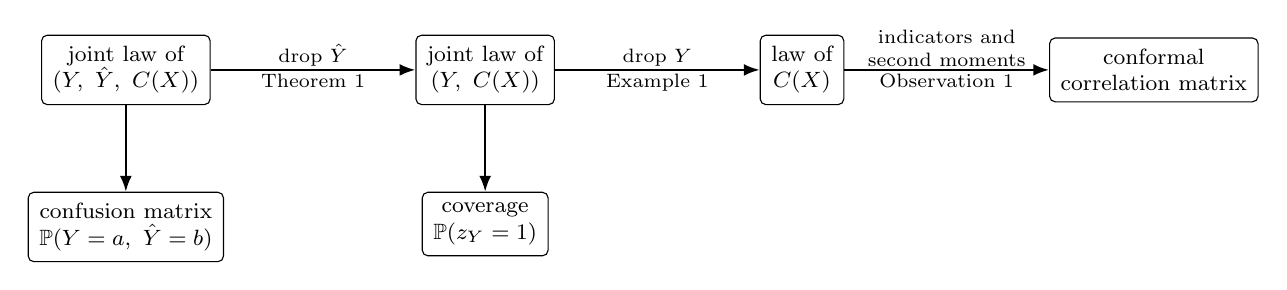
\begin{tikzpicture}[
  node distance=11mm and 26mm,
  box/.style={draw, rounded corners=2pt, inner sep=4pt, font=\footnotesize, align=center},
  lab/.style={font=\scriptsize, align=center, inner sep=1pt},
  arr/.style={-{Latex[length=2mm]}, thick}
]
\node[box] (full) {joint law of\\$(Y,\ \hat Y,\ C(X))$};
\node[box, right=of full] (yc) {joint law of\\$(Y,\ C(X))$};
\node[box, right=of yc] (c) {law of\\$C(X)$};
\node[box, right=of c] (ccm) {conformal\\correlation matrix};
\node[box, below=of full] (conf) {confusion matrix\\$\Prob(Y = a,\ \hat Y = b)$};
\node[box, below=of yc] (cov) {coverage\\$\Prob(z_Y = 1)$};
\draw[arr] (full) -- node[lab, above] {drop $\hat Y$} node[lab, below] {Theorem 1} (yc);
\draw[arr] (yc) -- node[lab, above] {drop $Y$} node[lab, below] {Example 1} (c);
\draw[arr] (c) -- node[lab, above] {indicators and\\second moments} node[lab, below] {Observation 1} (ccm);
\draw[arr] (full) -- (conf);
\draw[arr] (yc) -- (cov);
\end{tikzpicture}
\end{document}
